\def\xnode{\node[align=left, draw,thick,circle,black,minimum size=1.0cm,fill=gray!20!white]}
\def\znode{\node[align=left, draw,thick,circle,black,minimum size=1.0cm,fill=white]}

% IMPORTANT: define relative positions of the subpanels here.  Allows easy shuffling.

\begin{tikzpicture}[scale=1, >=triangle 45, triangle/.style = {fill=white, regular polygon, regular polygon sides=3 }]%,transform canvas={scale=0.8}]

% panel B 
 \node[triangle, draw=black, thick,inner sep=3mm](d0) at (2.7,-0.4) {}; 
% TRIANGLE PICTURES HERE
 \node (t0) at (2.7 - 0.024,-0.4+0.2) {
\includegraphics[width=18.5mm]{figs/fig1/t0.png}};  % include a picture here

 \node[triangle, draw=black, thick,inner sep=3mm](d1) at (1.0,-2.3) {}; 
  \node[triangle, draw=black, thick,inner sep=3mm](d2) at (2.7,-2.3) {}; 
   \node[triangle, draw=black, thick,inner sep=3mm](d3) at (4.4,-2.3) {};  
% TRIANGLE PICTURES HERE
 \node (t11) at (1.0 - 0.024,-2.3+0.2) {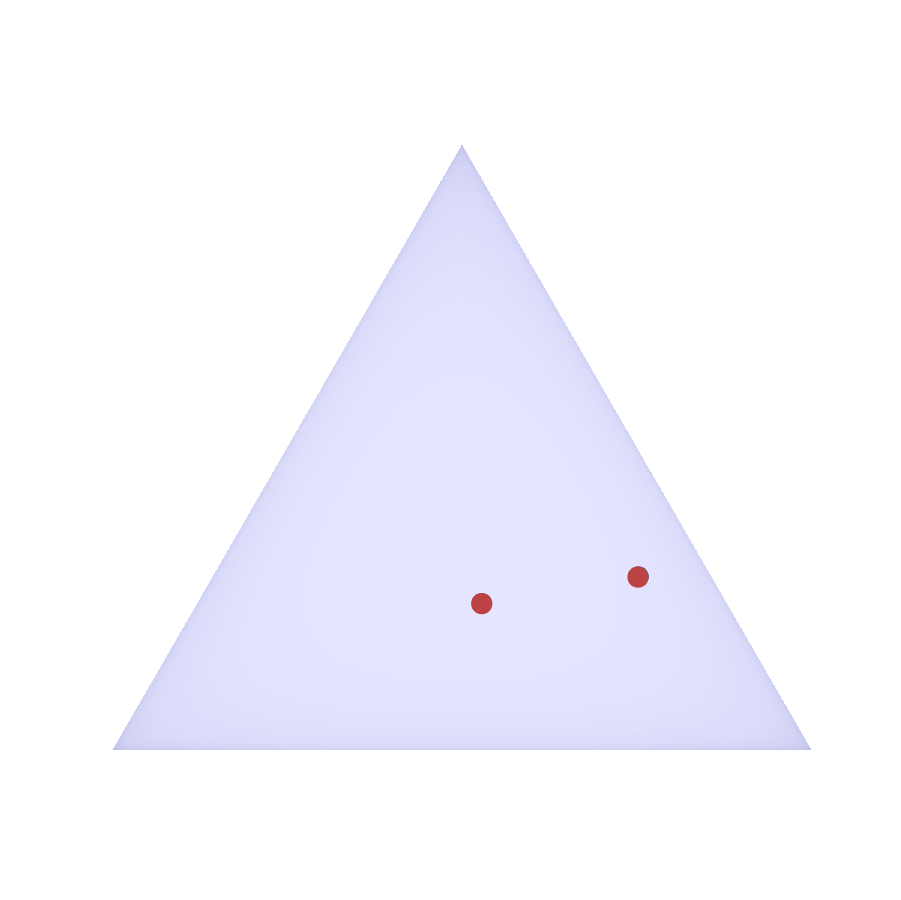
\includegraphics[width=18.5mm]{figs/fig1/t11a.png}};  % include a picture here
 \node (t12) at (2.7 - 0.024,-2.3+0.2) {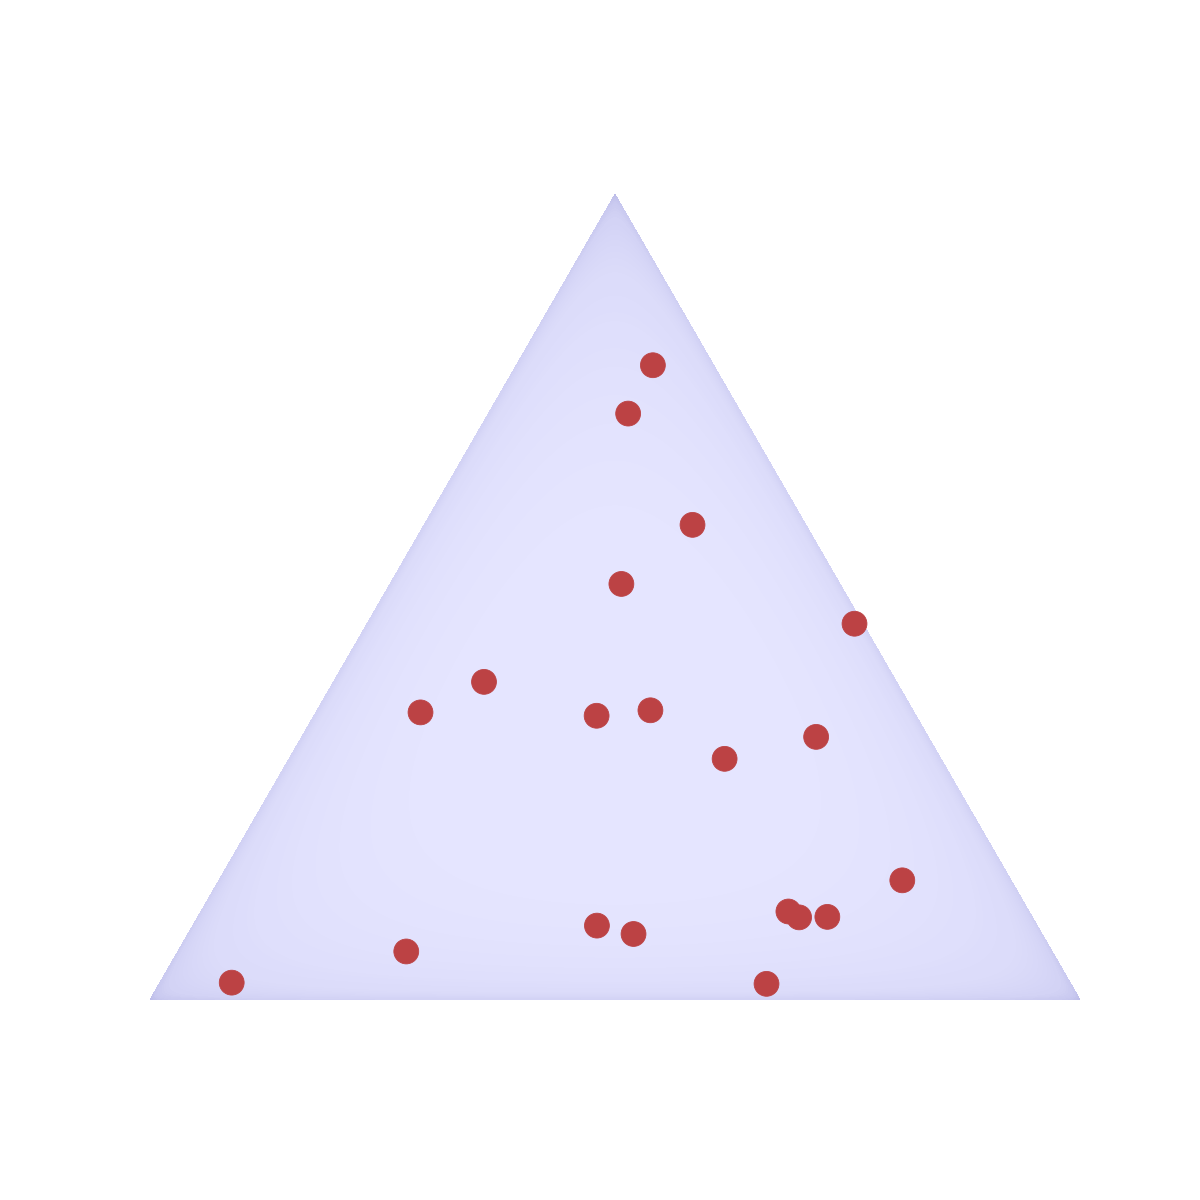
\includegraphics[width=18.5mm]{figs/fig1/t12.png}};  % include a picture here
 \node (t13) at (4.4 - 0.024,-2.3+0.2) {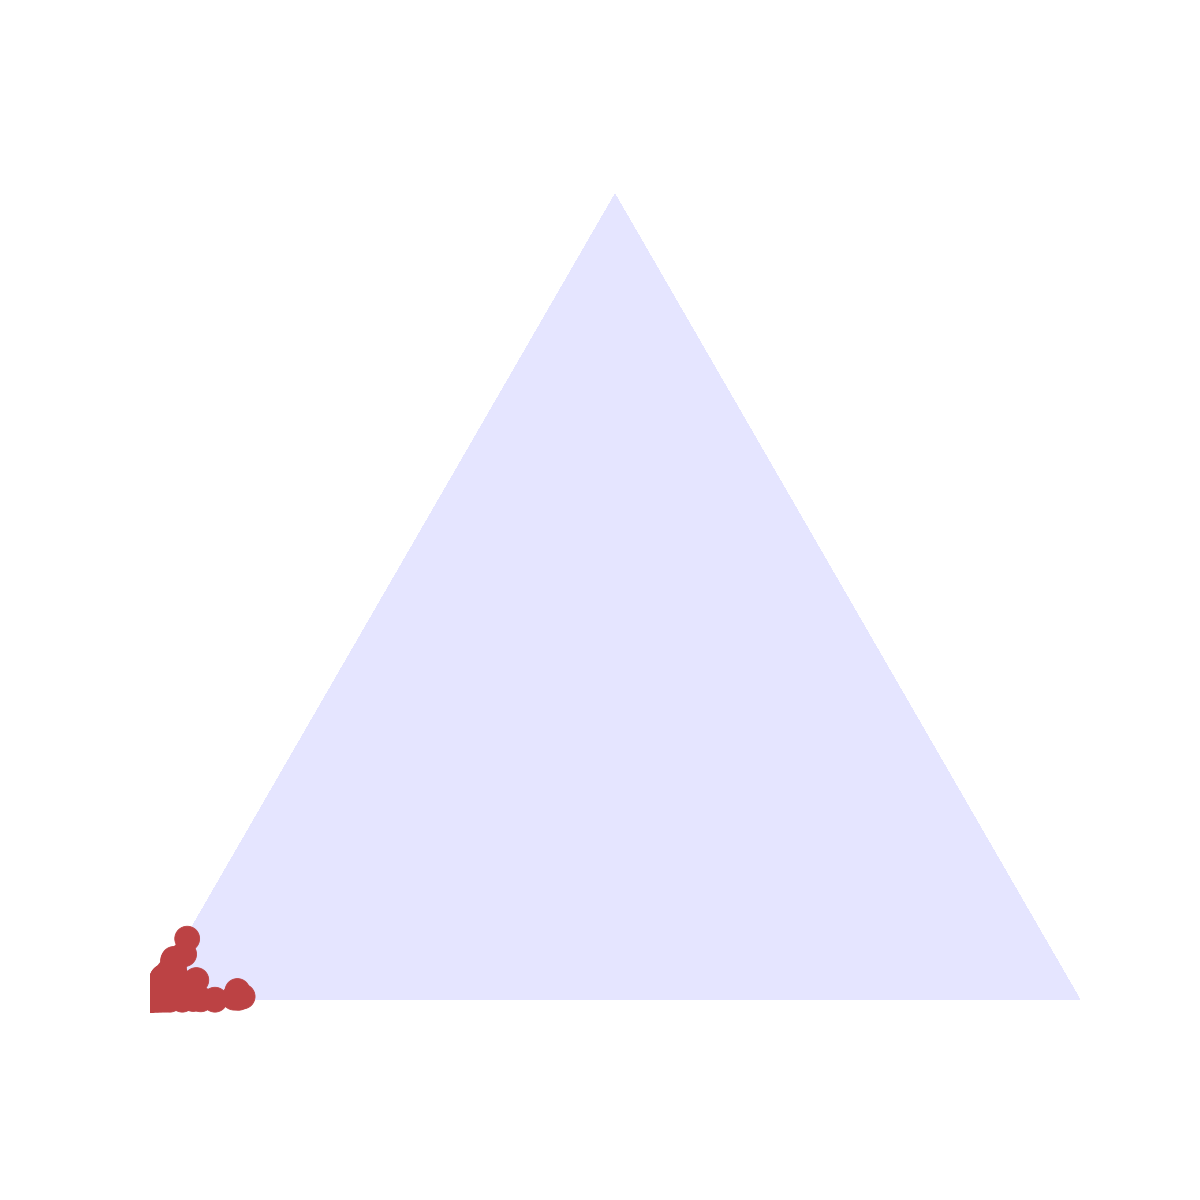
\includegraphics[width=18.5mm]{figs/fig1/t13.png}};  % include a picture here

  \node (dt) at (3.5,-2.1){...};

 \node[triangle, draw=black, thick,inner sep=3mm](dp1) at (1.0,-4.7) {}; 
  \node[triangle, draw=black, thick,inner sep=3mm](dp2) at (2.7,-4.7) {}; 
   \node[triangle, draw=black, thick,inner sep=3mm](dp3) at (4.4,-4.7) {};  
% TRIANGLE PICTURES HERE
 \node (t21) at (1.0 - 0.024,-4.7+0.2) {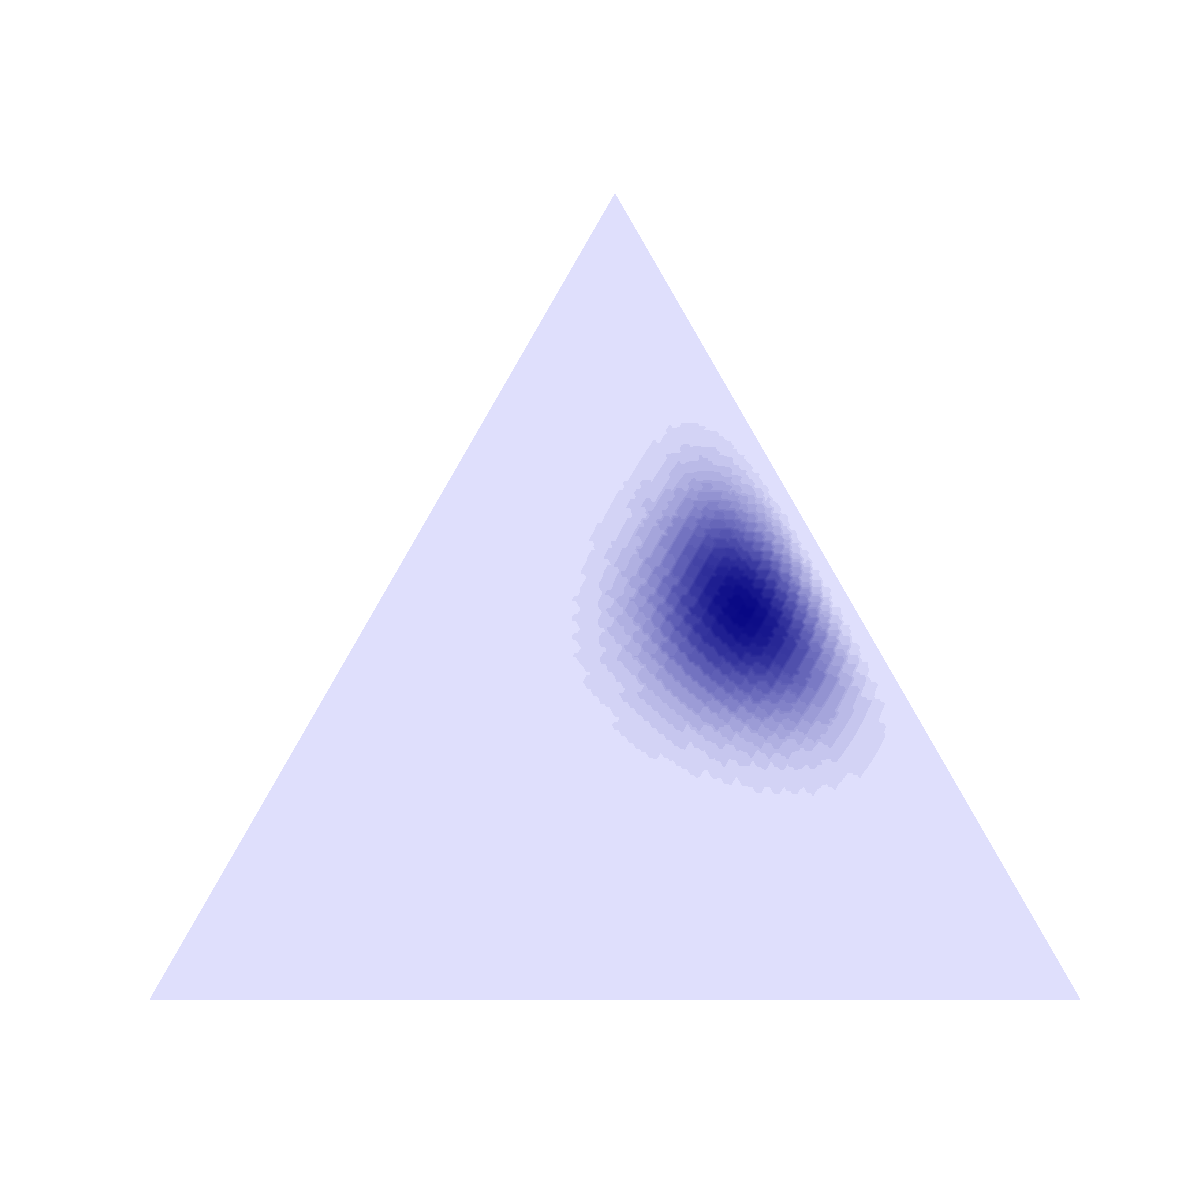
\includegraphics[width=18.5mm]{figs/fig1/t21.png}};  % include a picture here
 \node (t22) at (2.7 - 0.024,-4.7+0.2) {
\includegraphics[width=18.5mm]{figs/fig1/t22.png}};  % include a picture here
 \node (t23) at (4.4 - 0.024,-4.7+0.2) {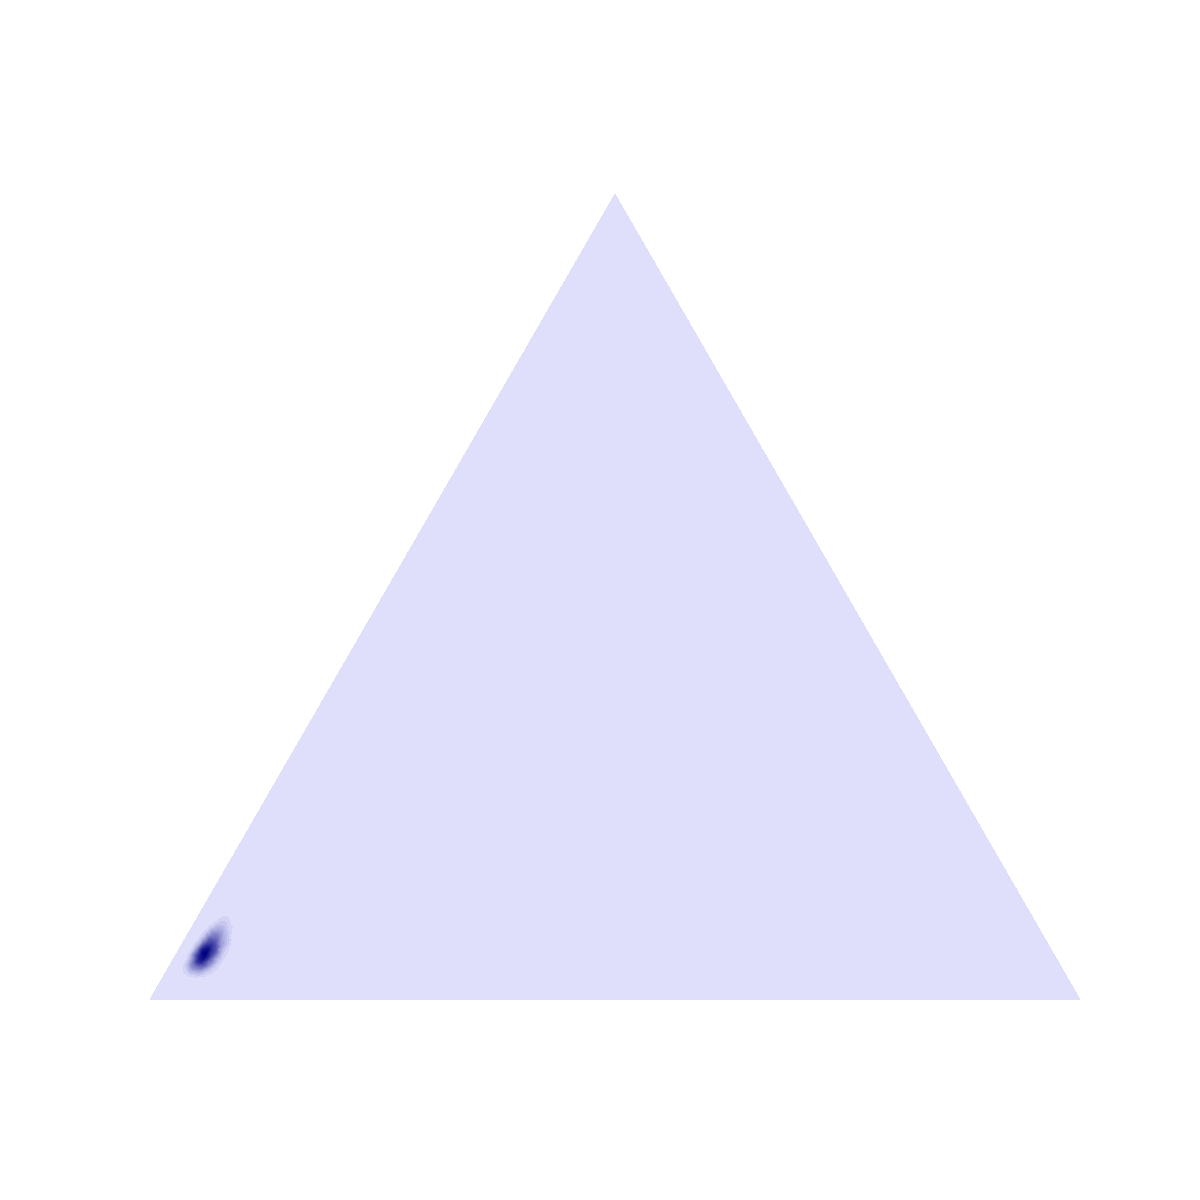
\includegraphics[width=18.5mm]{figs/fig1/t23.png}};  % include a picture here

  \node (dpt) at (3.5,-4.3){...};

 \node (p1) at (1.0,-2.8) {};
  \node (p2) at (2.7,-2.8) {};
   \node (p3) at (4.4,-2.8) {};
\draw[thick,dashed,-{Latex[length=0.5cm]}] (p1)--(dp1); 
\draw[thick,dashed,-{Latex[length=0.5cm]}] (p2)--(dp2); 
\draw[thick,dashed,-{Latex[length=0.5cm]}] (p3)--(dp3); 

\draw[thick,-{Latex[length=0.5cm]}] (d0.south)--(d1.north); 
\draw[thick,-{Latex[length=0.5cm]}] (d0.south)--(d2.north); 
\draw[thick,-{Latex[length=0.5cm]}] (d0.south)--(d3.north); 

  
\end{tikzpicture}
